\documentclass[11pt,a4paper]{report}

\usepackage{mathpazo}
\usepackage{microtype}
\usepackage{titlesec}
\usepackage{url}
\usepackage{graphicx}
\usepackage{verbatim}
\usepackage{epic}

\usepackage{tikz}
\usetikzlibrary{external}
\tikzexternalize[prefix=tikz/]

% Use stealth arrows
\tikzset {
  >=stealth
}

% Space out array environment
\newcommand*{\spacearray}{
\renewcommand{\arraystretch}{1.2}
\setlength{\arraycolsep}{4pt}
}

\textwidth=15cm
\textheight=23cm
\topmargin=12pt
\headheight=0pt
\oddsidemargin=2em
\headsep=0pt
\renewcommand{\baselinestretch}{1.1}
\setlength{\parskip}{0.2\baselineskip plus 1pt minus 1pt}
\parindent=0pt

\titleformat{\chapter}[display]{\normalfont\huge\bfseries}{\chaptertitlename\ \thechapter}{10pt}{\Huge}   
\titlespacing*{\chapter}{0pt}{-20pt}{20pt}
\titleformat{\section}[block]{\normalfont\Large\bfseries}{\thesection}{8pt}{\Large}
\setcounter{tocdepth}{1}

\begin{document}
\thispagestyle{empty}

\begin{center}
\begin{huge}
\begin{bfseries}
A Tutorial on Euler Angles and Quaternions
\end{bfseries}
\end{huge}

\bigskip
\bigskip
\bigskip

{\LARGE Moti Ben-Ari}

\bigskip

{\Large Department of Science Teaching\\
Weizmann Institute of Science\\
\bigskip
\url{http://www.weizmann.ac.il/sci-tea/benari/}
}

\bigskip
\bigskip


\begin{Large}
Version 2.0
\end{Large}
\end{center}

\vfill

\begin{center}
\copyright{}\  2014--17 by Moti Ben-Ari.
\end{center}

This work is licensed under the Creative Commons Attribution-ShareAlike 3.0 Unported License. To view a copy of this license, visit \url{http://creativecommons.org/licenses/by-sa/3.0/} or send a letter to Creative Commons, 444 Castro Street, Suite 900, Mountain View, California, 94041, USA.

\begin{center}

\includegraphics[width=.2\textwidth]{by-sa.png}
\end{center}

\clearpage
\setcounter{page}{1}

\chapter{Introduction}\label{s.intro}

You sitting in an airplane at night, watching a movie displayed on the screen attached to the seat in front of you. The airplane gently banks to the left. You may feel the slight acceleration, but you won't see any change in the position of the movie screen. Both you and the screen are in the same \emph{frame of reference}, so unless you stand up or make another move, the position and orientation of the screen relative to your position and orientation won't change. The same is not true with respect to your position and orientation relative to the frame of reference of the earth. The airplane is moving forward at a very high speed and the bank changes your orientation with respect to the earth.

The transformation of coordinates (position and orientation) from one frame of reference is a fundamental operation in several areas: flight control of aircraft and rockets, movement of manipulators in robotics, and computer graphics. This tutorial introduces the mathematics of rotations using two formalisms: (1) \emph{Euler angles} are the angles of rotation of a three-dimensional coordinate frame. A rotation of Euler angles is represented as a matrix of trigonometric functions of the angles. (2) \emph{Quaternions} are an algebraic structure that extends the familiar concept of complex numbers. While quaternions are much less intuitive than angles, rotations defined by quaternions can be computed more efficiently and with more stability, and therefore are widely used.

The tutorial assumes an elementary knowledge of trigonometry and matrices. The computations will be given in great detail for two reasons. First, so that you can be convinced of the correctness of the formulas, and, second, so that you can learn how to do them yourselves, in case you come across a context that uses different definitions or notation.

For a comprehensive presentation of quaternions using vector algebra, see: John Vince. \textit{Quaternions for Computer Graphics}, 2011, Springer.


%%%%%%%%%%%%%%%%%%%%%%%%%%%%%%%%

\chapter{Rotations in two dimensions}


We start by discussing rotations in two dimensions; the concepts and formulas should be familiar and a review will facilitate learning about rotations in three dimensions.

\section{Cartesian and polar coordinates}

A vector or a position (the tip of the vector) in a two-dimensional space can be given either in cartesian coordinates $(x,y)$ or in polar coordinates $(r,\phi)$, relative to a frame of reference:
\begin{center}
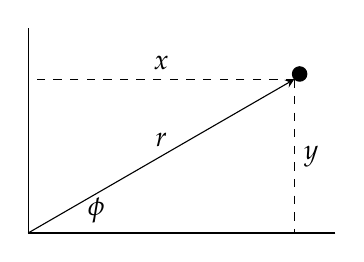
\begin{tikzpicture}[scale=1.3]
\draw (3,0) -- (0,0) coordinate (origin) -- (0,2);
\draw[->] (origin) node[right,xshift=18pt,yshift=8pt] {$\phi$} -- node[above] {$r$} (30:3) coordinate (point);
\draw[fill] (point) circle [radius=2pt,xshift=1.5pt,yshift=1.5pt];
\draw[dashed] (point) -- node[right,midway] {$y$} (point |- origin);
\draw[dashed] (point) -- node[above,midway] {$x$} (point -| origin);
\end{tikzpicture}
\end{center}

The formulas for transforming one representation to another are:
\begin{eqnarray*}
x &=& r \cos \phi\\
y &=& r \sin \phi\\
r &=& \sqrt{x^2 + y^2}\\
\phi &=& \tan^{-1}\,\frac{y}{x}\,.
\end{eqnarray*}

%%%%%%%%%%%%%%%%%%%%%%%%%%%%%%%%

\section{Rotating a vector}\label{s.rotating-vector}

Suppose now that the vector is rotated by the angle $\theta$:

\begin{center}
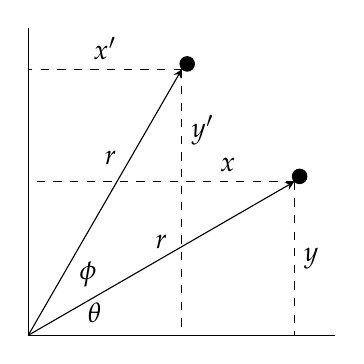
\begin{tikzpicture}[scale=1.3]
\draw (3,0) -- (0,0) coordinate (origin) -- (0,3);
% Before rotation
\draw[->] (origin) node[right,xshift=18pt,yshift=8pt] {$\theta$} -- node[above] {$r$} (30:3) coordinate (point1);
\draw[fill] (point1) circle [radius=2pt,xshift=1.5pt,yshift=1.5pt];
\draw[dashed] (point1) -- node[right,midway] {$y$} (point1 |- origin);
\draw[dashed] (point1) -- node[above,near start] {$x$} (point1 -| origin);
% After rotation
\draw[->] (origin) node[right,xshift=15pt,yshift=22pt] {$\phi$} -- node[above,xshift=2pt,yshift=10pt] {$r$} (60:3) coordinate (point2);
\draw[fill] (point2) circle [radius=2pt,xshift=1.5pt,yshift=1.5pt];
\draw[dashed] (point2) -- node[right,near start,yshift=2pt] {$y'$} (point2 |- origin);
\draw[dashed] (point2) -- node[above,midway] {$x'$} (point2 -| origin);
\end{tikzpicture}
\end{center}

The new vector's polar coordinates are $(r,\phi+\theta)$ and its cartesian coordinates can be computed using the trigonometric identities for the sum of two angles:
\begin{eqnarray*}
x' &=& r \cos(\phi + \theta)\\
&=& r (\cos\phi\cos\theta - \sin\phi\sin\theta)\\
&=& (r \cos\phi)\cos\theta - (r\sin\phi)\sin\theta\\
&=& x \cos\theta - y \sin\theta,\\
&& \mbox{}\\
y' &=& r \sin(\phi + \theta)\\
&=& r (\sin\phi\cos\theta + \cos\phi\sin\theta)\\
&=& (r \sin\phi)\cos\theta + (r \cos\phi)\sin\theta\\
&=& y \cos\theta + x \sin\theta\\
&=&  x \sin\theta + y \cos\theta\,.
\end{eqnarray*}
The transformation of the position $(x,y)$ to $(x',y')$ caused by a rotation through the angle $\theta$ can be expressed in matrix notation  as:
\[
\left[ 
\begin{array}{c} x'\\ y' \end{array}
\right] = 
\left[\begin{array}{l} \cos\theta \\ \sin\theta \end{array}\\
\begin{array}{l} -\sin\theta \\ \cos\theta \end{array}\\
\right]
\left[\begin{array}{l} x \\ y \end{array}\\
\right]\,.
\]

%%%%%%%%%%%%%%%%%%%%%%%%%%%%%%%%

\textbf{Example}

Let $r=1$ and let both $\theta$ and $\phi$ be $30^\circ$ so that:
\[
\begin{array}{l}
x=r\cos\phi = \cos \phi = \cos \theta = \cos 30^\circ = \sqrt{3}/2\\
y=r\sin\phi = \sin \phi = \sin \theta = \sin 30^\circ = 1/2\,.
\end{array}
\]
We can now compute the values of $x'$ and $y'$:
\begin{displaymath}
\left[ 
\begin{array}{c} x'\\ y' \end{array}
\right] = 
\left[\begin{array}{l} \sqrt{3}/2 \\ 1/2 \end{array}\\
\begin{array}{l} -1/2 \\ \sqrt{3}/2 \end{array}\\
\right]
\left[\begin{array}{l} \sqrt{3}/2 \\ 1/2 \end{array}\\ \right] =
\left[\begin{array}{l} (\sqrt{3}/2)^2 - (1/2)^2 \\ 1/2\cdot \sqrt{3}/2+1/2\cdot \sqrt{3}/2 \end{array}\\ \right] =
\left[\begin{array}{l} 1/2 \\ \sqrt{3}/2 \end{array}\\ \right]\,.
\end{displaymath}
The result makes sense since $\phi+\theta=60^\circ$.

%%%%%%%%%%%%%%%%%%%%%%%%%%%%%%%%

\section{A geometric derivation of the rotation matrix}

The rotation matrix can be derived geometrically. Rather than look at the vector, let us look at its $x$ and $y$ components and rotate them (counterclockwise) by $\theta$ (Figure~\ref{fig.geo}).

\begin{figure}
\begin{center}
\begin{tikzpicture}[scale=1.3]
\draw (0,0) coordinate (origin) node[left] {$O$} -- node[below] {$x\cos \theta$} (5,0) coordinate (x) node[right] {$A$} -- (5,3.5) coordinate (y);
\draw[fill] (y) circle [radius=2pt] node[right] {$B=(x,y)$};
\node[xshift=28pt,yshift=8pt] at (origin) {$\theta$};
\begin{scope}[rotate=30]
\draw (0,0) coordinate (origin) -- node[below] {$x$} (5,0) coordinate (x1) node[right] {$A'$} -- node[right] {$y$} (5,3.5) coordinate (y1);
\draw[fill] (y1) circle [radius=2pt] node[right] {$B'=(x',y')$};
\node[xshift=7pt,yshift=-24pt] at (y1) {$\theta$};
\node[above left,xshift=-5pt] at (x1) {$90-\theta$};
\end{scope}
\draw[fill] (x1-|y1) node[left] {$C'$} coordinate (int) circle [radius=1pt];
\draw[fill] (x1|-origin) node[below] {$C$} circle [radius=1pt];
\draw[dashed] (x1) -- node[left,midway] {$x\sin \theta$} (origin -| x1);
\draw[dashed] (x1) -- node[xshift=-8pt,below,midway] {$y\sin \theta$} (int);
\draw[dashed] (y1) -- node[left,midway] {$y\cos \theta$} (int);
\end{tikzpicture}
\caption{Geometric derivation of the rotation matrix}\label{fig.geo}
\end{center}
\end{figure}

The $x$- and $y$- components are rotated by the angle $\theta$ so that the $OAB$ becomes $OA'B'$. Construct two right triangles: (1) Drop the perpendicular from $A'$ to the $x$-axis to form the right triangle $\triangle OA'C$; (b) Construct a line through $A'$ parallel to the $x$-axis and a line through $B'$ parallel to the $y$-axis. They intersect at $C'$ to form the right triangle $\triangle B'A'C'$.

Since $A'C'$ is parallel to $CO$, $\angle C'A'O = \angle A'OC = \theta$. $\angle OA'B'$ is a right angle and $\triangle A'B'C'$ is a right triangle so $\angle A'B'C' = \theta$. The sides of the two right triangles are labeled with their lengths obtained by trigonometry. It is now easy to see that $x'$ is the length of $OC$ minus the length of $A'C'$ and that $y'$ is the length of $CA'$ plus the length of $C'B'$:
\begin{eqnarray*}
x' &=& x \cos\theta - y \sin\theta\\
y' &=& x \sin\theta + y \cos\theta.
\end{eqnarray*}

%%%%%%%%%%%%%%%%%%%%%%%%%%%%%%%%

\section{Rotating the frame of reference}

The effect of rotating a vector by $\theta$ is the same as the effect obtained by rotation of the frame of reference. The left diagram below shows a vector in the frame of reference $A$. The right diagram shows the same vector after frame $A$ is rotated $\theta$ relative to a new frame $B$.

\begin{center}
\begin{tikzpicture}[scale=1.3,baseline=-15pt]
\draw (3,0) node[right] {$x_A$} -- (0,0) coordinate (origin) -- (0,2) node[left] {$y_A$};
\draw[->,densely dashed] (origin) node[right,xshift=18pt,yshift=8pt] {$\phi$} -- node[above] {$r$} (30:3) coordinate (point);
\draw[fill] (point) circle [radius=2pt,xshift=1.5pt,yshift=1.5pt] node[above right] {$(x_A,y_A)$};
\end{tikzpicture}
\hspace{3em}
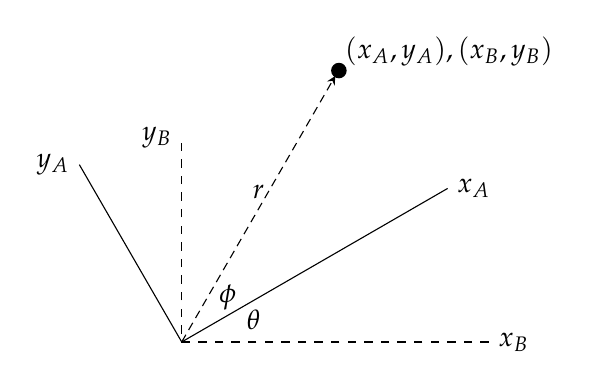
\begin{tikzpicture}[scale=1.3]
\draw[dashed] (3,0) node[right] {$x_B$} -- (0,0) coordinate (origin) -- (0,2) node[left] {$y_B$};
\draw[->,rotate=30,densely dashed] (origin) node[above right,xshift=10pt,yshift=8pt] {$\phi$} -- node[above] {$r$} (30:3) coordinate (point);
\draw[fill] (point) circle [radius=2pt,xshift=1pt,yshift=1.5pt] node[above right] {$(x_A,y_A),(x_B,y_B)$};
\draw[rotate=30] (3,0) node[right] {$x_A$} -- (0,0) node[right,xshift=20pt,yshift=8pt] {$\theta$} -- (0,2) node[left] {$y_A$};
\end{tikzpicture}
\end{center}

Given the coordinates $(x_A,y_A)$ of the points in the frame $A$:
\begin{eqnarray*}
x_A &=& r \cos \phi\\
y_A &=& r \sin \phi,
\end{eqnarray*}
what are its coordinates $(x_B,y_B)$ in the frame $B$? The geometry of this diagram is the same as the geometry of the diagram in Section~\ref{s.rotating-vector}, so we can use the same equation:

\begin{equation}
\left[ 
\begin{array}{c} x_B\\ y_B \end{array}
\right] = 
\left[\begin{array}{l} \cos\theta \\ \sin\theta \end{array}\\
\begin{array}{l} -\sin\theta \\ \cos\theta \end{array}\\
\right]
\left[\begin{array}{l} x_A \\ y_A \end{array}\\
\right].
\end{equation}

%%%%%%%%%%%%%%%%%%%%%%%%%%%%%%%%

\textbf{Example}

Consider the point $(x_A,y_A) = (\sqrt{3}/2,1/2)$ in frame $A$. What are the coordinates of the point in frame $B$? As before, the computation gives:
\begin{displaymath}
\left[ 
\begin{array}{c} x_B\\ y_B \end{array}
\right] = 
\left[\begin{array}{l} \sqrt{3}/2 \\ 1/2 \end{array}\\
\begin{array}{l} -1/2 \\ \sqrt{3}/2 \end{array}\\
\right]
\left[\begin{array}{l} \sqrt{3}/2 \\ 1/2 \end{array}\\ \right] =
\left[\begin{array}{l} 1/2 \\ \sqrt{3}/2 \end{array}\\ \right].
\end{displaymath}

%%%%%%%%%%%%%%%%%%%%%%%%%%%%%%%%

\section{Multiple rotations}

Rotate the coordinate frame $B$ by $\psi$ relative to a new frame $C$.
\begin{center}
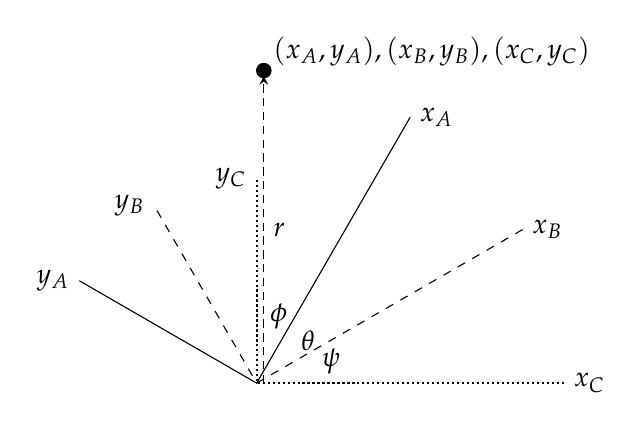
\begin{tikzpicture}[scale=1.3]
\draw[thick,densely dotted] (3,0) node[right] {$x_C$} -- (0,0) coordinate (origin) -- (0,2) node[left] {$y_C$};
\draw[->,densely dashed] (2pt,0) node[above right,xshift=10pt,yshift=8pt] {$\theta$} -- node[right] {$r$} (2pt,3) coordinate (point);
%\draw[->,rotate=60,densely dashed] (origin) node[above right,xshift=10pt,yshift=8pt] {$\psi$} -- node[right] {$r$} (30:3) coordinate (point);
\draw[fill] (point) circle [radius=2pt,yshift=1.5] node[above right] {$(x_A,y_A),(x_B,y_B),(x_C,y_C)$};
\draw[rotate=30,dashed] (3,0) node[right] {$x_B$} -- (0,0) node[right,xshift=20pt,yshift=8pt] {$\psi$} -- (0,2) node[left] {$y_B$};
\draw[rotate=60] (3,0) node[right] {$x_A$} -- (0,0) node[above,xshift=8pt,yshift=16pt] {$\phi$} -- (0,2) node[left] {$y_A$};
\end{tikzpicture}
\end{center}
If we know $(x_B,y_B)$, we can multiply it by the rotation matrix for $\psi$ to obtain $(x_C,y_C)$.

Let us denote the rotation matrix from frame $A$ to frame $B$ by $R^B_A$ and the rotation matrix from frame $B$ to frame $C$ by $R^C_B$. Given $p^A$, the coordinates of a point in frame $A$, its coordinates in frame $B$ are $p^B=R^B_A p^A$, and $p^C$, its coordinates in frame $C$, are $p^C=R^C_B p^B$. Combining the two equations we have:
\[
p^C = R^C_B p^B = R^C_B R^B_A p^A\,.
\]
Let $R^C_A = R^C_B R^B_A$. This is the rotation matrix from $A$ to $C$, so we can obtain the coordinates $p^C$ directly from $p^A$ by:
\[
p^C = R^C_A p^A\,.
\]

\pagebreak[3]

\textbf{Example}

Let $\psi=30^\circ$ so $R^C_B=R^B_A$. Then:
\begin{displaymath}
\spacearray
\left[ 
\begin{array}{c} x_C\\ y_C \end{array}
\right] = 
\left[\begin{array}{l} \sqrt{3}/2 \\ 1/2 \end{array}\\
\begin{array}{l} -1/2 \\ \sqrt{3}/2 \end{array}\\
\right]
\left[\begin{array}{l} 1/2 \\ \sqrt{3}/2 \end{array}\\ \right] =
\left[\begin{array}{l} 0 \\ 1 \end{array}\\ \right]\,.
\end{displaymath}
From the drawing we see the vector lies on the $y_C$-axis which corresponds to the coordinates $(0,1)$.

Let us now compute:
\[
\spacearray
R^C_A=R^C_B R^B_A = 
\left[\begin{array}{l} \sqrt{3}/2 \\ 1/2 \end{array}\\
\begin{array}{l} -1/2 \\ \sqrt{3}/2 \end{array}\\
\right]
\left[\begin{array}{l} \sqrt{3}/2 \\ 1/2 \end{array}\\
\begin{array}{l} -1/2 \\ \sqrt{3}/2 \end{array}\\
\right]=
\left[\begin{array}{l} 1/2 \\ \sqrt{3}/2 \end{array}\\
\begin{array}{l} -\sqrt{3}/2 \\ 1/2\end{array}\\
\right]\,.
\]
The computation $p^C = R^C_A p^A$ is:
\[\spacearray
\left[ 
\begin{array}{c} x_C\\ y_C \end{array}
\right] =
\left[\begin{array}{l} 1/2 \\ \sqrt{3}/2 \end{array}\\
\begin{array}{l} -\sqrt{3}/2 \\ 1/2\end{array}\\
\right]
\left[\begin{array}{l} \sqrt{3}/2 \\ 1/2\end{array}\\ \right]\\ =
\left[\begin{array}{l} 0 \\ 1 \end{array}\\ \right]\,,
\]
the same result obtained in the two-stage computation.

%%%%%%%%%%%%%%%%%%%%%%%%%%%%%%%%

\textbf{Example}

Consider the vector $(1,0)$ lying on the $x$-axis of frame $A$. Rotate $A$ by $15^\circ$ to frame $B$ and then rotate frame $B$ by $30^\circ$ to frame $C$. Hopefully, the coordinates of the vector in frame $C$ will be $(\sqrt{2}/2,\sqrt{2}/2)$, because the vector makes an angle of $45^\circ$ with the $x$-axis of frame $C$.

The values of the trigonometric functions for $15^\circ$ are:
\[\cos 15^\circ = \frac{\sqrt{6}+\sqrt{2}}{4},\;\;\; \sin 15^\circ\frac{\sqrt{6}-\sqrt{2}}{4}\,.
\]

First rotate by $15^\circ$:
\begin{displaymath}
\spacearray
\left[ 
\begin{array}{c} x_B\\ y_B \end{array}
\right] = 
\left[
\begin{array}{l} \frac{\sqrt{6}+\sqrt{2}}{4} \\ \frac{\sqrt{6}-\sqrt{2}}{4} \end{array}\\
\begin{array}{l} -\frac{\sqrt{6}-\sqrt{2}}{4} \\ \frac{\sqrt{6}+\sqrt{2}}{4} \end{array}\\
\right]
\left[\begin{array}{l} 1 \\ 0 \end{array}\\ \right] =
\left[
\begin{array}{l} \frac{\sqrt{6}+\sqrt{2}}{4} \\ \frac{\sqrt{6}-\sqrt{2}}{4} \end{array}\\
\right]\,.
\end{displaymath}
Now rotate by $30^\circ$:
\begin{displaymath}
\spacearray
\left[ 
\begin{array}{c} x_C\\ y_C \end{array}
\right] = 
\left[
\begin{array}{l} \frac{\sqrt{3}}{2} \\ \frac{1}{2} \end{array}\\
\begin{array}{l} -\frac{1}{2} \\ \frac{\sqrt{3}}{2} \end{array}\\
\right]
\left[
\begin{array}{l} \frac{\sqrt{6}+\sqrt{2}}{4} \\ \frac{\sqrt{6}-\sqrt{2}}{4} \end{array}\\
\right]=
\left[
\begin{array}{l} \frac{\sqrt{18}+\sqrt{2}}{8} \\ \frac{\sqrt{18}+\sqrt{2}}{8} \end{array}\\
\right]=
\left[
\begin{array}{l} \frac{\sqrt{2}}{2} \\ \frac{\sqrt{2}}{2} \end{array}\\
\right]\,.
\end{displaymath}
If we multiply the two rotation matrices:
\begin{displaymath}
\spacearray
\left[
\begin{array}{l} \frac{\sqrt{6}+\sqrt{2}}{4} \\ \frac{\sqrt{6}-\sqrt{2}}{4} \end{array}\\
\begin{array}{l} -\frac{\sqrt{6}-\sqrt{2}}{4} \\ \frac{\sqrt{6}+\sqrt{2}}{4} \end{array}\\
\right]
\left[
\begin{array}{l} \frac{\sqrt{3}}{2} \\ \frac{1}{2} \end{array}\\
\begin{array}{l} -\frac{1}{2} \\ \frac{\sqrt{3}}{2} \end{array}\\
\right]=
\left[
\begin{array}{l} \frac{\sqrt{2}}{2} \\ \frac{\sqrt{2}}{2} \end{array}\\
\begin{array}{l} -\frac{\sqrt{2}}{2} \\ \frac{\sqrt{2}}{2} \end{array}\\
\right]\,,
\end{displaymath}
the result is the rotation matrix for a rotation by $45^\circ$.

If we multiply the two matrices in the opposite order, we get the same result:
\begin{displaymath}
\spacearray
\left[
\begin{array}{l} \frac{\sqrt{3}}{2} \\ \frac{1}{2} \end{array}\\
\begin{array}{l} -\frac{1}{2} \\ \frac{\sqrt{3}}{2} \end{array}\\
\right]
\left[
\begin{array}{l} \frac{\sqrt{6}+\sqrt{2}}{4} \\ \frac{\sqrt{6}-\sqrt{2}}{4} \end{array}\\
\begin{array}{l} -\frac{\sqrt{6}-\sqrt{2}}{4} \\ \frac{\sqrt{6}+\sqrt{2}}{4} \end{array}\\
\right]
=
\left[
\begin{array}{l} \frac{\sqrt{2}}{2} \\ \frac{\sqrt{2}}{2} \end{array}\\
\begin{array}{l} -\frac{\sqrt{2}}{2} \\ \frac{\sqrt{2}}{2} \end{array}\\
\right]\,.
\end{displaymath}
This shows that rotating by $15^\circ$ and then by $30^\circ$ gives the same result as rotating by $30^\circ$ and then by $15^\circ$. This is not surprising because we are familiar with the commutativity of turning knobs clockwise and counterclockwise. Unfortunately, we will not be so lucky when we discuss three-dimensional rotations.

%%%%%%%%%%%%%%%%%%%%%%%%%%%%%%%%

\chapter{Rotations in three dimensions}

The concept of coordinate transformations in three-dimensions is the same as in two dimensions, however, the mathematics are more complicated. Furthermore, many of us find it difficult to visualize explanations of three-dimensional motion when all we are shown is two-dimensional representations of three-dimensional objects.

The great eighteenth-century mathematician Leonhard Euler proved that an arbitrary three-dimensional rotation can be obtained by three individual rotations around the axes. In his honor, the angles of the rotations are called \emph{Euler angles}. 

\section{Rotations around the three axes}

A two-dimensional $x$-$y$ coordinate frame can be considered to be part of the three-dimensional coordinate frame by adding a $z$-axis perpendicular to the $x$- and $y$-axes. Here is a two-dimensional representation of the three-dimensional coordinate frame:
%\begin{figure}
\begin{center}
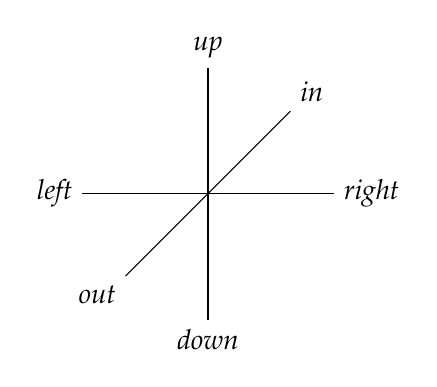
\begin{tikzpicture}[scale=.8]
\draw (-2,0,0) node [left] {\textit{left}} -- (2,0,0) node [right] {\textit{right}};
\draw (0,-2,0) node [below] {\textit{down}} -- (0,2,0) node [above] {\textit{up}};
\draw (0,0,-3.4) node [above right] {\textit{in}} -- (0,0,3.4) node [below left] {\textit{out}};
\end{tikzpicture}
%\caption{Three-dimensional coordinate frame}\label{fig.frame}
\end{center}
%\end{figure}
The $x$-axis is drawn left and right on the paper and the $y$-axis is drawn up and down on the paper. The diagonal line represents the $z$-axis, which is perpendicular to the other two axes and therefore its positive direction is out of the paper and its negative direction is into the paper.

The standard $x$-$y$-$z$ coordinate frame has the positive directions of its axes pointing in the directions (\textit{right}, \textit{up}, \textit{out}) as shown in the left diagram:
%\begin{figure}
\begin{center}
\begin{tikzpicture}
\draw [->] (0,0,0) -- (2,0,0) node [right] {$x$};
\draw [->] (0,0,0) -- (0,2,0) node [above] {$y$};
\draw [->] (0,0,0) -- (0,0,2) node [below left] {$z$};
\draw[->] (.5,0,1) arc [start angle=0, end angle=270, radius=3.5mm];
\end{tikzpicture}
\hspace{3em}
\begin{tikzpicture}
\draw [->] (0,0,0) -- (-2,0,0) node [left] {$y$};
\draw [->] (0,0,0) -- (0,2,0) node [above] {$x$};
\draw [->] (0,0,0) -- (0,0,2) node [below left] {$z$};
\end{tikzpicture}
%\caption{Rotation around the $z$-axis}\label{fig.rotatez}
\end{center}
%\end{figure}
Rotate the coordinate frame counterclockwise around the $z$-axis, so the $z$-axis which remains unchanged (right diagram). The new orientation of the frame is (\textit{up}, \textit{left}, \textit{out}).

Consider now a rotation of $90^\circ$ around the $x$-axis:
%\begin{figure}
\begin{center}
\begin{tikzpicture}
\draw [->] (0,0,0) -- (2,0,0) node [right] {$x$};
\draw [->] (0,0,0) -- (0,2,0) node [above] {$y$};
\draw [->] (0,0,0) -- (0,0,2) node [below left] {$z$};
\draw[->] (1.4,.1,0) arc [start angle=0, end angle=270, radius=3.5mm];
\end{tikzpicture}
\hspace{3em}
\begin{tikzpicture}[baseline=-4em]
\draw [->] (0,0,0) -- (2,0,0) node [right] {$x$};
\draw [->] (0,0,0) -- (0,-2,0) node [below] {$z$};
\draw [->] (0,0,0) -- (0,0,2) node [below left] {$y$};
\end{tikzpicture}
%\caption{Rotation around the $x$-axis}\label{fig.rotatex}
\end{center}
%\end{figure}
This causes the $y$-axis to ``jump out'' of the page and the $z$-axis to ``fall down'' onto the page, resulting in the orientation (\textit{right}, \textit{out}, \textit{down}).

Finally, consider a rotation of $90^\circ$ around the $y$-axis (left diagram):
%\begin{figure}
\begin{center}
\begin{tikzpicture}
\draw [->] (0,0,0) -- (2,0,0) node [right] {$x$};
\draw [->] (0,0,0) -- (0,2,0) node [above] {$y$};
\draw [->] (0,0,0) -- (0,0,2) node [below left] {$z$};
\draw[->] (.7,1,.6) arc [start angle=0, end angle=270, radius=3.5mm];
\end{tikzpicture}
\hspace{3em}
\begin{tikzpicture}[baseline=-3.8em]
\draw [->] (0,0,0) -- (2,0,0) node [right] {$z$};
\draw [->] (0,0,0) -- (0,2,0) node [above] {$y$};
\draw [->] (0,0,0) -- (0,0,-2) node [above right] {$x$};
\end{tikzpicture}
%\caption{Rotation around the $y$-axis}\label{fig.rotatey}
\end{center}
%\end{figure}
The $x$-axis ``drops below'' the paper and the $z$-axis ``falls right'' onto the paper. The new position of the frame is (\textit{in}, \textit{up}, \textit{right}).

\section{The right hand rule}

The $z$-axis must be perpendicular to the $x$- and $y$-axes, but there are two orientations for this line: one in which the positive direction of the axis is out of the paper and another where the positive direction of the axis is into the paper. It doesn't matter which one we choose as long as the choice is consistent.

The conventional choice is the \emph{right hand rule}. Curl the fingers of your right hand so that they go by the shortest path from the one axis to another axis. Your thumb now points in the positive direction of the third axis. For the familiar $x$- and $y$-axes on paper, curl your fingers on the short $90^\circ$ path from the $x$-axis to the $y$-axis (\emph{not} on the long $270^\circ$ path from the $x$-axis to the $y$-axis). When you do so your thumb points out of the paper and this is taken as the positive direction of the $z$-axis.

The following diagram shows the right-hand coordinate system displayed with each of the three axes pointing out of the paper:
\begin{center}
\begin{tikzpicture}[scale=.8]
\draw [->] (0,0,0) -- (2,0,0) node [right] {$x$};
\draw [->] (0,0,0) -- (0,2,0) node [above] {$y$};
\draw [->] (0,0,0) -- (0,0,2) node [below left] {$z$};
\draw[->] (.5,0,1) arc [start angle=0, end angle=270, radius=3.5mm];
\end{tikzpicture}
\hspace{2em}
\begin{tikzpicture}[scale=.8]
\draw [->] (0,0,0) -- (2,0,0) node [right] {$y$};
\draw [->] (0,0,0) -- (0,2,0) node [above] {$z$};
\draw [->] (0,0,0) -- (0,0,2) node [below left] {$x$};
\draw[->] (.5,0,1) arc [start angle=0, end angle=270, radius=3.5mm];
\end{tikzpicture}
\hspace{2em}
\begin{tikzpicture}[scale=.8]
\draw [->] (0,0,0) -- (2,0,0) node [right] {$z$};
\draw [->] (0,0,0) -- (0,2,0) node [above] {$x$};
\draw [->] (0,0,0) -- (0,0,2) node [below left] {$y$};
\draw[->] (.5,0,1) arc [start angle=0, end angle=270, radius=3.5mm];
\end{tikzpicture}
\end{center}

The three rotations are:
\begin{quote}
\normalsize
Rotate from x to y around z,\\
Rotate from y to z around x,\\
Rotate from z to x around y.
\end{quote}

\section{Matrices for three-dimensional rotations}

A three-dimensional rotation matrix will be a $3\times 3$ matrix because each point $p$ in a frame has three coordinates $p_x,p_y,p_z$ that must be moved. Consider first a rotation around the $z$-axis. The $x$ and $y$ coordinates are rotated as in two dimensions and the $z$ coordinate remains unchanged. Therefore, the matrix is:
\[
\spacearray
\left[\begin{array}{ccc}\cos\theta&-\sin\theta&0\\\sin\theta&\cos\theta&0\\0&0&1\end{array}\right]\,.
\]
For a rotation about the $x$-axis, the $x$ coordinate is unchanged and the $y$ and $z$ coordinates are transformed ``as if'' they were the $x$ and $y$ coordinates of a rotation around the $z$-axis:
\[
\spacearray
\left[\begin{array}{ccc}1&0&0\\0&\cos\theta&-\sin\theta\\0&\sin\theta&\cos\theta\\\end{array}\right]\,.
\]
For a rotation about the $y$-axis, the $y$ coordinate is unchanged and the $z$ and $x$ coordinates are transformed ``as if'' they were the $x$ and $y$ coordinates of a rotation around the $z$-axis:
\[
\spacearray
\left[\begin{array}{ccc}\cos\theta&0&\sin\theta\\0&1&0\\-\sin\theta&0&\cos\theta\\\end{array}\right]\,.
\]
It may seem strange that the signs of $\sin\theta$ have changed. To convince yourself that this matrix is correct, redraw the diagram in Section~\ref{s.rotating-vector} and perform the computations, substituting $z$ for $x$ and $x$ for $y$.

\section{Multiple rotations}\label{s.multiple-rotations}

Here is an example of three successive rotations of a coordiante frame: first, $90^\circ$ around the $z$-axis, then $90^\circ$ around the $y$-axis and finally $90^\circ$ around the $x$-axis:
\begin{center}
\begin{tikzpicture}[scale=.7]
\draw [->] (0,0,0) -- (2,0,0) node [right] {$x$};
\draw [->] (0,0,0) -- (0,2,0) node [above] {$y$};
\draw [->] (0,0,0) -- (0,0,2) node [below left] {$z$};
\draw[->] (0,-.3,.1) arc [start angle=0, end angle=270, radius=3mm];
\end{tikzpicture}
\hspace{2em}
\begin{tikzpicture}[scale=.7]
\draw [->] (0,0,0) -- (-2,0,0) node [left] {$y$};
\draw [->] (0,0,0) -- (0,2,0) node [above] {$x$};
\draw [->] (0,0,0) -- (0,0,2) node [below left] {$z$};
\draw[<-] (-.6,.1,0) arc [start angle=0, end angle=270, radius=3mm];
\end{tikzpicture}
\hspace{2em}
\begin{tikzpicture}[scale=.7,baseline=-3em]
\draw [->] (0,0,0) -- (0,2,0) node [above] {$z$};
\draw [->] (0,0,0) -- (-2,0,0) node [left] {$y$};
\draw [->] (0,0,0) -- (0,0,-2.5) node [above right] {$x$};
\draw[<-] (.6,.2,-.5) arc [start angle=0, end angle=270, radius=3mm];
\end{tikzpicture}
\hspace{2em}
\begin{tikzpicture}[scale=.7,baseline=-3em]
\draw [->] (0,0,0) -- (0,2,0) node [above] {$y$};
\draw [->] (0,0,0) -- (2,0,0) node [right] {$z$};
\draw [->] (0,0,0) -- (0,0,-2.5) node [above right] {$x$};
\end{tikzpicture}
\end{center}
This is called a $zyx$ Euler angle rotation. The final orientation is (\textit{in}, \textit{up}, \textit{right}).

There is one caveat to composing rotations: three-dimensional rotations \emph{do not} commute. Let us demonstrate this by a simple sequence of two rotations. Consider a rotation of $90^\circ$ around the $z$-axis, followed by a rotation of $90^\circ$ around the $x$-axis:
\begin{center}
\begin{tikzpicture}[scale=.8]
\draw [->] (0,0,0) -- (2,0,0) node [right] {$x$};
\draw [->] (0,0,0) -- (0,2,0) node [above] {$y$};
\draw [->] (0,0,0) -- (0,0,2) node [below left] {$z$};
\draw[->] (.5,0,1) arc [start angle=0, end angle=270, radius=3.5mm];
\end{tikzpicture}
\hspace{2em}
\begin{tikzpicture}[scale=.8]
\draw [->] (0,0,0) -- (-2,0,0) node [left] {$y$};
\draw [->] (0,0,0) -- (0,2,0) node [above] {$x$};
\draw [->] (0,0,0) -- (0,0,2) node [below left] {$z$};
\draw[->] (.7,1,.6) arc [start angle=0, end angle=270, radius=3.5mm];
\end{tikzpicture}
\hspace{2em}
\begin{tikzpicture}[scale=.8]
\draw [->] (0,0,0) -- (2,0,0) node [right] {$z$};
\draw [->] (0,0,0) -- (0,2,0) node [above] {$x$};
\draw [->] (0,0,0) -- (0,0,2) node [below left] {$y$};
\end{tikzpicture}
\end{center}
The result can be expressed as (\textit{up}, \textit{out}, \textit{right}).

Now consider the commuted operation: a rotation of $90^\circ$ around the $x$-axis, followed by a rotation of $90^\circ$ around the $z$-axis:
\begin{center}
\begin{tikzpicture}[scale=.8]
\draw [->] (0,0,0) -- (2,0,0) node [right] {$x$};
\draw [->] (0,0,0) -- (0,2,0) node [above] {$y$};
\draw [->] (0,0,0) -- (0,0,2) node [below left] {$z$};
\draw[->] (1.4,.1,0) arc [start angle=0, end angle=270, radius=3.5mm];
\end{tikzpicture}
\hspace{2em}
\begin{tikzpicture}[scale=.8,baseline=-3.1em]
\draw [->] (0,0,0) -- (2,0,0) node [right] {$x$};
\draw [->] (0,0,0) -- (0,0,2) node [below left] {$y$};
\draw [->] (0,0,0) -- (0,-2,0) node [below] {$z$};
\draw[<-] (.7,-1,.6) arc [start angle=0, end angle=270, radius=3.5mm];
\end{tikzpicture}
\hspace{2em}
\begin{tikzpicture}[scale=.8,baseline=-3em]
\draw [->] (0,0,0) -- (0,0,2) node [below left] {$x$};
\draw [->] (0,0,0) -- (-2,0,0) node [left] {$y$};
\draw [->] (0,0,0) -- (0,-2,0) node [below] {$z$};
\end{tikzpicture}
\end{center}
The result can be expressed as (\textit{out}, \textit{left}, \textit{down}) which is not the same as the previous orientation.

There are three axes so there should be $3^3=27$ sequences of Euler angles. However, there is no point in rotating around the same axis twice in succession because the same result can be obtained by rotating once by the sum of the angles, so there are only $3\cdot 2\cdot 2=12$ different Euler angle sequences:
\[
\begin{array}{cccc}
xyx & xyz & xzx & xzy \\
yxy & yxz & yzx & yzy \\
zxy & zxz & zyx & zyz\,.
\end{array}
\]

\section{Euler angles for transforming a vector}

Let us return to the sequence of Euler angle rotations at the beginning of Section~\ref{s.multiple-rotations}. Consider the vector (or point) $(1,1,1)$ in the final frame:
\begin{center}
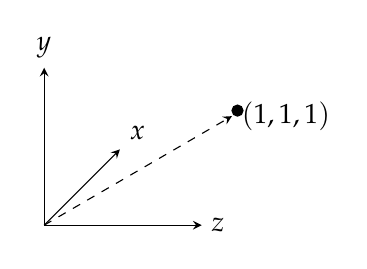
\begin{tikzpicture}
\draw [->] (0,0,0) -- (0,2,0) node [above] {$y$};
\draw [->] (0,0,0) -- (2,0,0) node [right] {$z$};
\draw [->] (0,0,0) -- (0,0,-2.5) node [above right] {$x$};
\draw[->,dashed] (0,0,0) -- (2,1,-1) node[right] {$(1,1,1)$};
\draw[fill] (2,1,-1) circle [xshift=2pt,yshift=2pt,radius=2pt];
\end{tikzpicture}
\end{center}
What are its coordinates in the previous frame that was rotated around the $x$-axis to become this frame? Rotating the previous frame (\emph{not} the vector), we find that the point's coordinates are $(1,-1,1)$:
\begin{center}
\begin{tikzpicture}[scale=.7]
\draw [->] (0,0,0) -- (0,2,0) node [above] {$z$};
\draw [->] (0,0,0) -- (-2,0,0) node [left] {$y$};
\draw [->] (0,0,0) -- (0,0,-2.5) node [above right] {$x$};
\draw[<-] (.6,.2,-.8) arc [start angle=0, end angle=270, radius=3mm];
\draw[->,dashed] (0,0,0) -- (2,1,-1) node[right] {$(1,-1,1)$};
\draw[fill] (2,1,-1) circle [xshift=2pt,yshift=2pt,radius=2pt];
\end{tikzpicture}
\end{center}
What are its coordinates in the previous frame that was rotated around the $y$-axis to become this frame? Rotating the previous frame around the $y$-axis gives $(1,-1,-1)$:
\begin{center}
\begin{tikzpicture}[scale=.7]
\draw [->] (0,0,0) -- (-2,0,0) node [left] {$y$};
\draw [->] (0,0,0) -- (0,2,0) node [above] {$x$};
\draw [->] (0,0,0) -- (0,0,2) node [below left] {$z$};
\draw[<-] (-.6,.1,0) arc [start angle=0, end angle=270, radius=3mm];
\draw[->,dashed] (0,0,0) -- (2,1,-1) node[right] {$(1,-1,-1)$};
\draw[fill] (2,1,-1) circle [xshift=2pt,yshift=2pt,radius=2pt];
\end{tikzpicture}
\end{center}
Finally, what are its coordinates in the previous frame that was rotated around the $z$-axis to become this frame? Rotating the previous frame around the $z$-axis gives the coordinates in the original frame $(1,1-,1)$:
\begin{center}
\begin{tikzpicture}[scale=.7]
\draw [->] (0,0,0) -- (2,0,0) node [right] {$x$};
\draw [->] (0,0,0) -- (0,2,0) node [above] {$y$};
\draw [->] (0,0,0) -- (0,0,2) node [below left] {$z$};
\draw[->] (0,-.3,.1) arc [start angle=0, end angle=270, radius=3mm];
\draw[->,dashed] (0,0,0) -- (2,1,-1) node[right] {$(1,1,-1)$};
\draw[fill] (2,1,-1) circle [xshift=2pt,yshift=2pt,radius=2pt];
\end{tikzpicture}
\end{center}

These coordinates can be computed from the rotation matrices for the rotations around the three axes. First around the $x$-axis:
\[
\spacearray
\left[\begin{array}{c}1\\-1\\1\end{array}\right] =
\left[\begin{array}{ccc}1&0&0\\0&0&-1\\0&1&0\\\end{array}\right]
\left[\begin{array}{c}1\\1\\1\end{array}\right]\,,
\]
then around the $y$-axis:
\[
\spacearray
\left[\begin{array}{c}1\\-1\\-1\end{array}\right] =
\left[\begin{array}{ccc}0&0&1\\0&1&0\\-1&0&0\\\end{array}\right]
\left[\begin{array}{c}1\\-1\\1\end{array}\right]\,,
\]
and finally around the $z$-axis:
\[
\spacearray
\left[\begin{array}{c}1\\1\\-1\end{array}\right] =
\left[\begin{array}{ccc}0&-1&0\\1&0&0\\0&0&1\\\end{array}\right]
\left[\begin{array}{c}1\\-1\\-1\end{array}\right]\,.
\]

%%%%%%%%%%%%%%%%%%%%%%%%%%%%%%%%

\section{One matrix for three rotations}

Instead of performing the three multiplications of a vector by a matrix, we can multiply the matrices for the three Euler angles together. The result is the matrix for the complete rotation:
\[
\spacearray
\begin{scriptstyle}
\left[\begin{array}{ccc}0&-1&0\\1&0&0\\0&0&1\\\end{array}\right]
\left(
\left[\begin{array}{ccc}0&0&1\\0&1&0\\-1&0&0\\\end{array}\right]
\left[\begin{array}{ccc}1&0&0\\0&0&-1\\0&1&0\\\end{array}\right]
\right)
=
\left[\begin{array}{ccc}0&-1&0\\1&0&0\\0&0&1\\\end{array}\right]
\left[\begin{array}{ccc}0&1&0\\0&0&-1\\-1&0&0\\\end{array}\right]
=
\left[\begin{array}{ccc}0&0&1\\0&1&0\\-1&0&0\\\end{array}\right]\,.
\end{scriptstyle}
\]
The vector $(1,1,1)$ can now be multiplied by this matrix and we obtain the expected value:
\[
\spacearray
\left[\begin{array}{c}1\\1\\-1\end{array}\right]
=
\left[\begin{array}{ccc}0&0&1\\0&1&0\\-1&0&0\\\end{array}\right]
\left[\begin{array}{c}1\\1\\1\end{array}\right]\,.
\]

%%%%%%%%%%%%%%%%%%%%%%%%%%%%%%%%

\section{The matrix for an arbitrary rotation}

The previous section showed an example of a matrix that rotates a vector around the axes $zyx$ by $90^\circ$ each. The matrix for arbitrary rotations around these axes is obtained by multiplying the matrices for each axis using arbitrary angles: a rotation of $\psi$ around the $z$-axis, a rotation of $\theta$ around the $y$ axis and a rotation of $\phi$ around the $x$-axis. The resulting matrix is computed as follows. First multiply the rotation around the $x$-axis by the rotation around the $y$-axis:
\[
\spacearray
\begin{scriptstyle}
R_{y(\theta)} \, R_{x(\phi)} =
\left[
\begin{array}{ccc}
\cos\theta & 0 & \sin\theta\\
0 & 1 & 0\\
-\sin\theta &0& \cos\theta\\
\end{array}
\right]
\left[
\begin{array}{ccc}
1&0&0\\
0&\cos\phi & -\sin\phi\\
0&\sin\phi & \cos\phi\\
\end{array}
\right]
=
\left[
\begin{array}{lll}
\cos\theta  &  \sin\theta\sin\phi & \sin\theta\cos\phi \\
0& \cos\phi & -\sin\phi\\
-\sin\theta & \cos\theta\sin\phi &  \cos\theta\cos\phi\\
\end{array}
\right]\,.
\end{scriptstyle}
\]
Then, multiply the result by the rotation around the $z$-axis:
\[
\spacearray
\begin{scriptstyle}
R_{z(\psi)y(\theta)x(\phi)}=R_{z(\psi)}\,(R_{y(\theta)} \, R_{x(\phi)}) =
\left[
\begin{array}{ccc}
\cos\psi & -\sin\psi &0\\
\sin\psi & \cos\psi &0\\
0&0&1\\
\end{array}
\right]
\left[
\begin{array}{lll}
\cos\theta  &  \sin\theta\sin\phi & \sin\theta\cos\phi \\
0& \cos\phi & -\sin\phi\\
-\sin\theta & \cos\theta\sin\phi &  \cos\theta\cos\phi\\
\end{array}
\right]\,.
\end{scriptstyle}
\]

\[
\spacearray
\begin{scriptstyle}
R_{z(\psi)y(\theta)x(\phi)}=R_{z(\psi)}\,(R_{y(\theta)} \, R_{x(\phi)}) =
\left[
\begin{array}{lll}
% First row
\cos\psi\cos\theta  &  \cos\psi\sin\theta\sin\phi- & \cos\psi\sin\theta\cos\phi+ \\
                    &  \sin\psi\cos\phi & \sin\psi\sin\phi\\
\\
% Second row
\sin\psi\cos\theta &\sin\psi\sin\theta\sin\phi+ & \sin\psi\sin\theta\cos\phi-\\
&\cos\psi\cos\phi  &\cos\psi\sin\phi\\
\\
% Third row
-\sin\theta & \cos\theta\sin\phi& \cos\theta\cos\phi\\
\end{array}
\right]\,.
\end{scriptstyle}
\]

For the rotation $R_{z(90)y(90)x(90)}$, we can evaluate the matrix to obtain the matrix we computed from the individual rotations:
\[
\spacearray
\left[\begin{array}{ccc}0&0&1\\0&1&0\\-1&0&0\\\end{array}\right]\,.
\]

%%%%%%%%%%%%%%%%%%%%%%%%%%%%%%%%

\chapter{Quaternions}

\section{Complex numbers}

A complex number is a pair written formally as $a+bi$, where $a,b$ are real numbers and $i$ is a new symbol. Arithmetic is performed as if complex numbers were formal polynomials with indeterminate $i$ and then simplified using the identify $i^2=-1$:
\begin{eqnarray*}
(a+bi) + (c+di) &=& (a+c) + (b+d)i\\
(a+bi)\,(c+di) &=& ac + adi + bci + bdi^2\\
&=&(ac-bd) + (ad+bc)i.
\end{eqnarray*}
Complex numbers can represent vectors and points in the plane. The number $x+iy$ is identified with the vector from $(0,0)$ to the point $(x,y)$. Complex multiplication can be used to rotate a vector. By Euler's formula:
\[
e^{i\theta} = (\cos\theta + i\sin\theta)\,,
\]
so:
\[
e^{i\theta}(x+iy) = (\cos\theta + i\sin\theta)(x+yi)
=(x\cos\theta - y\sin\theta) + i(x\sin\theta+y\cos\theta)\,,
\]
which is the two-dimensional rotation of $(x,y)$ by $\theta$:
\begin{displaymath}
\left[ 
\begin{array}{c} x'\\ y' \end{array}
\right] = 
\left[\begin{array}{l} \cos\theta \\ \sin\theta \end{array}\\
\begin{array}{l} -\sin\theta \\ \cos\theta \end{array}\\
\right]
\left[\begin{array}{l} x \\ y \end{array}\\
\right]\,.
\end{displaymath}
In 1843, the mathematician William R. Hamilton discovered that three-dimensional rotations can be described by a generalization of complex numbers called quaternions.

\section{The algebra of quaternions}

A quaternion is a 4-tuple written formally as $q_0+q_1i+q_2j+q_3k$,
where $q_i$ are real numbers and the symbols $i,j,k$ satisfy the
following identities:
\begin{displaymath}
\begin{array}{l}
i^2=j^2=k^2=-1\\
ij=k,\,ji=-k\\
jk=i,\,kj=-i\\
ki=j,\,ik=-j\,.
\end{array}
\end{displaymath}
Multiplication of these symbols $i,j,k$ are \emph{not commutative}. To remember the sign of a multiplication, consider the symbols to be arranged cyclically:
\begin{center}
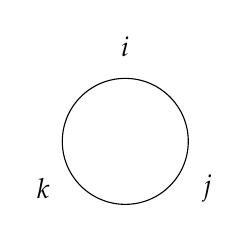
\begin{tikzpicture}
\draw (0,0) circle[radius=8mm];
\node at (90:1.2) {$i$};
\node at (210:1.2) {$k$};
\node at (330:1.2) {$j$};
\end{tikzpicture}
\end{center}
If two symbols to be multiplied are adjacent clockwise, the sign is plus, whereas if they are adjacent counterclockwise, the sign is minus.

Arithmetic is performed formally and the results are simplified using the identities. Here are the formulas for adding and multiplying two quaternions:
\begin{eqnarray*}
\lefteqn{(q_0+q_1i+q_2j+q_3k)+(p_0+p_1i+p_2j+p_3k)}\\
&=& (q_0+p_0) + (q_1+p_1)i + (q_2+p_2)j + (q_3+p_3)k\\
%
&\rule{0pt}{2pt}&\\
%
\lefteqn{(q_0+q_1i+q_2j+q_3k)\, (p_0+p_1i+p_2j+p_3k)}\\
&=& (q_0p_0 + q_1p_1i^2 + q_2p_2j^2+q_3p_3k^2) +\\
&& (q_0p_1i + q_1p_0i + q_2p_3jk + q_3p_2kj) +\\
&& (q_0p_2j + q_2p_0j + q_1p_3ik + q_3p_1ki) +\\
&& (q_0p_3k + q_3p_0k + q_1p_2ij + q_2p_1ji)\\
&=& (q_0p_0 - q_1p_1 - q_2p_2 - q_3p_3) +\\
&& (q_0p_1 + q_1p_0 + q_2p_3 - q_3p_2)i +\\
&& (q_0p_2 + q_2p_0 - q_1p_3 + q_3p_1)j +\\
&& (q_0p_3 + q_3p_0 + q_1p_2 - q_2p_1)k.
\end{eqnarray*}

\section{The conjugate and absolute value of a complex number}

Complex numbers form a \emph{field}, because multiplication is commutative and every nonzero complex number has an inverse:
\begin{eqnarray*}
(a+bi)(a-bi) &=& a^2 - b^2i^2 = a^2+b^2\\
\frac{(a+bi)(a-bi)}{a^2+b^2} &=& 1\\
(a+bi)^{-1} &=& \frac{a-bi}{a^2+b^2}\,.
\end{eqnarray*}
For a complex number $z=a+bi$, define its \emph{conjugate} $z^*$ as $a-bi$ and its \emph{norm} as $|z|=\sqrt{a^2+b^2}$. Then its inverse can be written as:
\begin{displaymath}
z^{-1}=\frac{z^*}{|z|^2}\,.
\end{displaymath}

\section{The conjugate and norm of a quaternion}

The corresponding definitions for quaternions are as follows.

Given $q=q_0+q_1i+q_2j+q_3k$, its \emph{conjugate} is:
\begin{displaymath}
q^*=q_0-q_1i-q_2j-q_3k\,,
\end{displaymath}
and its \emph{norm} is:
\begin{displaymath}
|q|=\sqrt{q_0^2+q_1^2+q_2^2+q_3^2}\,.
\end{displaymath}
Every nonzero quaternion has an inverse:
\begin{eqnarray*}
q\,q^* &=& (q_0+q_1i+q_2j+q_3k)(q_0-q_1i-q_2j-q_3k)\\
&=& (q_0q_0 - q_1q_1i^2 - q_2q_2j^2 - q_3q_3k^2) +\\
&& (-q_0q_1 + q_1q_0 - q_2q_3 + q_3q_2)i +\\
&& (-q_0q_2 + q_2q_0 + q_1q_3 - q_3q_1)j +\\
&& (-q_0q_3 + q_3q_0 - q_1q_2 + q_2q_1)k\\
&=&  q_0^2 + q_1^2 + q_2^2 + q_3^2\,.\\
q^{-1}&=&\frac{q^*}{|q|^2}\,.
\end{eqnarray*}
Quaternions do not form a field because multiplication is not commutative.

%%%%%%%%%%%%%%%%%%%%%%%%%%%%%%%%

\section{Quaternions for rotations}

A vector in three-dimensional space can be expressed as a \emph{pure quaternion}, a quaternion with no real part: $q = 0+xi+yj+zk$. A rotation is expressed by a quaternion $q_R$ with the additional requirement that its norm $|q_R|$ be equal to $1$. A rotation from one coordinate frame $A$ to another $B$ is given by the conjugation operation:

\begin{displaymath}
q_B = q_R \, q_A \,  q^*_R.
\end{displaymath}

This operation will result in a quaternion $q_B$ which is also a vector since it has no real part:
\begin{eqnarray*}
q_R \, q_A \,  q^*_R &=& (q_0+q_1i+q_2j+q_3k)(xi+yj+zk)(q_0-q_1i-q_2j-q_3k)\\
&=& (x(q_0^2+q_1^2-q_2^2-q_3^2)+2y(q_1q_2-q_0q_3)+2z(q_0q_2+q_1q_3))i +\\
&& (2x(q_0q_3+q_1q_2)+y(q_0^2-q_1^2+q_2^2-q_3^2)+2z(q_2q_3-q_0q_1))j +\\
&& (2x(q_1q_3-q_0q_2)+2y(q_0q_1+q_2q_3)+z(q_0^2-q_1^2-q_2^2+q_3^2))k.
\end{eqnarray*}

The detailed multiplication is given in Appendix~\ref{a.mult-quat}.

This computation does not require the computation of trigonometric functions, only the addition and multiplication of real numbers.

%%%%%%%%%%%%%%%%%%%%%%%%%%%%%%%%

\section{From a quaternion to a rotation matrix}

We need to compute the quaternion of a rotation from Euler angles and rotation matrices and conversely from quaternions back to angles and matrices.

Expressing the formula for $q_R \, q_A \,  q^*_R$ as a matrix gives:
\begin{displaymath}
\spacearray
M=
\left[
\begin{array}{lll}
q_0^2+q_1^2-q_2^2-q_3^2 & 2(q_1q_2-q_0q_3) & 2(q_0q_2+q_1q_3)\\
2(q_0q_3+q_1q_2) & q_0^2-q_1^2+q_2^2-q_3^2 & 2(q_2q_3-q_0q_1)\\
2(q_1q_3-q_0q_2) & 2(q_0q_1+q_2q_3) & q_0^2-q_1^2-q_2^2+q_3^2\\
\end{array}
\right].
\end{displaymath}

The matrix can be simplified since the norm of a rotation quaternion is $1$:
\begin{displaymath}
|q| = q_0^2+q_1^2+q_2^2+q_3^2 = 1,
\end{displaymath}
from which we have the following equations:
\begin{eqnarray*}
-q_2^2-q_3^2 &=& q_0^2+q_1^2-1\\
-q_1^2-q_3^2 &=& q_0^2+q_2^2-1\\
-q_1^2-q_2^2 &=& q_0^2+q_3^2-1.
\end{eqnarray*}
After simplification the matrix becomes:
\begin{displaymath}
\spacearray
M=
2\cdot\left[
\begin{array}{lll}
q_0^2+q_1^2-0.5 & q_1q_2-q_0q_3 & q_0q_2+q_1q_3\\
q_0q_3+q_1q_2 & q_0^2+q_2^2-0.5 & q_2q_3-q_0q_1\\
q_1q_3-q_0q_2 & q_0q_1+q_2q_3 & q_0^2+q_3^2-0.5\\
\end{array}
\right].
\end{displaymath}

\section{From a matrix of angles to a quaternion}\label{s.mtoq}

Given a rotation matrix $M$, we can compute the quaternion that represents the same rotation. First compute the \emph{trace}, the sum of the elements on the main diagonal of the matrix:
\begin{eqnarray*}
\textit{Trace}(M)&=&M_{11}+M_{22}+M_{33}\\
&=&2(3q_0^2+q_1^2+q_2^2+q_3^2-1.5)\\
&=&2(3q_0^2+(1-q_0^2)-1.5)\\
&=&2(2q_0^2-0.5)\\
&=&4q_0^2-1.
\end{eqnarray*}
We can solve this equation for $q_0$:
\begin{displaymath}
|q_0|=\sqrt{\frac{\textit{Trace}(M)+1}{4}}.
\end{displaymath}
Once we have $q_0$, we can obtain $q_1$ from $M_{11}$:
\begin{displaymath}
M_{11} = 2(q_0^2+q_1^2-0.5)=2\left(\frac{\textit{Trace}(M)+1}{4}+q_1^2-0.5\right).
\end{displaymath}
\begin{displaymath}
|q_1|=\sqrt{\frac{M_{11}}{2}+\frac{1-\textit{Trace}(M)}{4}}.
\end{displaymath}
Similarly, $q_2$ and $q_3$ can be computed from $M_{22}$ and $M_{33}$:
\begin{displaymath}
|q_2|=\sqrt{\frac{M_{22}}{2}+\frac{1-\textit{Trace}(M)}{4}}.
\end{displaymath}
\begin{displaymath}
|q_3|=\sqrt{\frac{M_{33}}{2}+\frac{1-\textit{Trace}(M)}{4}}.
\end{displaymath}


%%%%%%%%%%%%%%%%%%%%%%%%%%%%%%%%

\section{From Euler angles to a quaternion}\label{s.atoq}

Given a rotation by an angle, the corresponding quaternion can be computed. Consider the rotation $\psi$ around the $z$-axis:
\begin{displaymath}
\spacearray
M_\psi=\left[
\begin{array}{ccc}
\cos\psi & -\sin\psi & 0\\
\sin\psi & \cos\psi & 0\\
0&0&1\\
\end{array}
\right].
\end{displaymath}
From the formulas in the previous section and using that $\textit{Trace}(M)=2\cos\psi+1$:
\begin{eqnarray*}
|q_0|&=&\sqrt{\frac{2\cos\psi+1+1}{4}}=\sqrt{\frac{1+\cos\psi}{2}}=\cos\frac{\psi}{2},\\
&\rule{0pt}{4pt}&\\
|q_1|=|q_2|&=&\sqrt{\frac{\cos\psi}{2}+\frac{1-(2\cos\psi+1)}{4}}=0,\\
&\rule{0pt}{4pt}&\\
|q_3|&=&\sqrt{\frac{1}{2}+\frac{1-(2\cos\psi+1)}{4}}=\sqrt{\frac{1-\cos\psi}{2}}=\sin\frac{\psi}{2}.
\end{eqnarray*}
Therefore:
\begin{displaymath}
q_\psi=\cos\frac{\psi}{2} + k\sin\frac{\psi}{2}.
\end{displaymath}

Similarly, we can compute the quaternions corresponding to rotations around the $y$- and $x$-axes:
\begin{eqnarray*}
q_\theta&=&\cos\frac{\theta}{2} + j\sin\frac{\theta}{2},\\
&\rule{0pt}{4pt}&\\
q_\phi&=&\cos\frac{\phi}{2} + i\sin\frac{\phi}{2}.
\end{eqnarray*}

%%%%%%%%%%%%%%%%%%%%%%%%%%%%%%%%

\section{Example}

Consider a rotation of $+90^\circ$ around the $z$-axis. It takes the point $(1,0,0)$ to $(0,1,0)$. The rotation matrix is:
\begin{displaymath}
\spacearray
\left[
\begin{array}{ccc}
\cos 90^\circ & -\sin 90^\circ & 0\\
\sin 90^\circ & \cos 90^\circ & 0\\
0&0&1\\
\end{array}
\right] =
\left[
\begin{array}{ccc}
0 & -1 & 0\\
1  & 0 & 0\\
0&0&1\\
\end{array}
\right].
\end{displaymath}
Using the formulas in Section~\ref{s.mtoq} and computing $\textit{Trace}(M)=0+0+1=1$, we have:
\begin{eqnarray*}
|q_0|&=&\sqrt{\frac{\textit{Trace}(M)+1}{4}}=\sqrt{\frac{1+1}{4}}=
\sqrt{\frac{1}{2}}=\frac{\sqrt{2}}{2}\\
|q_1|&=&\sqrt{\frac{M_{11}}{2}+\frac{1-\textit{Trace}(M)}{4}}=
\sqrt{0+0}=0\\
|q_2|&=&\sqrt{\frac{M_{22}}{2}+\frac{1-\textit{Trace}(M)}{4}}=
\sqrt{0+0}=0\\
|q_3|&=&\sqrt{\frac{M_{33}}{2}+\frac{1-\textit{Trace}(M)}{4}}=
\sqrt{\frac{1}{2}+0}=\sqrt{\frac{1}{2}}=\frac{\sqrt{2}}{2}.
\end{eqnarray*}
Therefore:
\begin{displaymath}
q_R = \frac{\sqrt{2}}{2} - \frac{\sqrt{2}}{2}k.
\end{displaymath}
We can obtain the same result directly from the formula in Section~\ref{s.atoq}:
\begin{displaymath}
q_R = \cos 45^\circ + k\sin 45^\circ = \frac{\sqrt{2}}{2} + \frac{\sqrt{2}}{2}k. 
\end{displaymath}

The point $(1,0,0)$ is $0+i+0j+0k$ as a quaternion so we compute the rotation as:
\begin{eqnarray*}
\lefteqn{q_R\, i \, q_R^*}\\
&=&(\frac{\sqrt{2}}{2} + \frac{\sqrt{2}}{2}k)\, i \, (\frac{\sqrt{2}}{2} -
 \frac{\sqrt{2}}{2}k)\\
&=&(\frac{\sqrt{2}}{2}i + \frac{\sqrt{2}}{2}ki)\, (\frac{\sqrt{2}}{2} -
 \frac{\sqrt{2}}{2}k)\\
&=&(\frac{\sqrt{2}}{2}i + \frac{\sqrt{2}}{2}j)\, (\frac{\sqrt{2}}{2} -
 \frac{\sqrt{2}}{2}k)\\
&=&\frac{1}{2}(i+j-ik-jk)\\
&=&\frac{1}{2}(i+j+j-i)\\
&=&j.
\end{eqnarray*}
This is the point $(0,1,0)$ as expected.
%%%%%%%%%%%%%%%%%%%%%%%%%%%%%%%%

\appendix
\chapter{Multiplication of three quaternions}\label{a.mult-quat}

We compute the multiplication of quarternions to change a coordinate frame:
\begin{displaymath}
q_R \, q_A \,  q^*_R = (q_0+q_1i+q_2j+q_3k)(xi+yj+zk)(q_0-q_1i-q_2j-q_3k)\,.
\end{displaymath}
Multiply the first two factors:
\begin{eqnarray*}
\lefteqn{(q_0+q_1i+q_2j+q_3k)(xi+yj+zk)}\\
&=& q_0xi+q_0yj+q_0zk+\\
&& q_1xi^2+q_1yij+q_1zik+\\
&& q_2xji+q_2yj^2+q_2zjk+\\
&& q_3xki+q_3ykj+q_3zk^2\\
&=& -q_1x-q_2y-q_3z+\\
&& q_0xi+q_2zi-q_3yi+\\
&& q_0yj-q_1zj+q_3xj+\\
&& q_0zk+q_1yk-q_2xk\,.
\end{eqnarray*}
Now mulitply on the right by $(q_0-q_1i-q_2j-q_3k)$.

\textbf{The real part}

Multiply the first row by $q_0$, the second by $-q_1i$, the third by $-q_2j$ and the fourth by $-q_3k$:
\begin{displaymath}
\spacearray
\begin{array}{l}
-q_0q_1x-q_0q_2y-q_0q_3z\\
+q_0q_1x+q_1q_2z-q_1q_3y\\
+q_0q_2y-q_1q_2z+q_2q_3x\\
+q_0q_3z+q_1q_3y-q_2q_3x=0\,.
\end{array}
\end{displaymath}

\textbf{The coefficient of $i$}

Multiply the second row by $q_0$ the first by $-q_1i$, the fourth by $-q_2j$ (since $kj=-i$) and the third by $-q_3k$ (since $jk=i$):
\begin{displaymath}
\spacearray
\begin{array}{l}
+q_0q_0x+q_0q_2z-q_0q_3y\\
+q_1q_1x+q_1q_2y+q_1q_3z\\
+q_0q_2z+q_1q_2y-q_2q_2x\\
-q_0q_3y+q_1q_3z-q_3q_3x\,.
\end{array}
\end{displaymath}
Collecting terms gives:
\begin{displaymath}
\spacearray
\begin{array}{l}
(q_0^2+q_1^2-q_2^2-q_3^2)x+\\
2(q_1q_2-q_0q_3)y+\\
2(q_0q_2+q_1q_3)z\,.
\end{array}
\end{displaymath}

\textbf{The coefficient of $j$}

Multiply the third row by $q_0$, the fourth by $-q_1i$ (since $ki=j$),
the first by $-q_2j$ and the second by $-q_3k$ (since $ik=-j$):
\begin{displaymath}
\begin{array}{l}
+q_0q_0y-q_0q_1z+q_0q_3x\\
-q_0q_1z-q_1q_1y+q_1q_2x\\
+q_1q_2x+q_2q_2y+q_2q_3x\\
+q_0q_3x+q_2q_3z-q_3q_3y\,.
\end{array}
\end{displaymath}
Collecting terms gives:
\begin{displaymath}
\begin{array}{l}
2(q_1q_2+q_0q_3)x+\\
(q_0^2-q_1^2+q_2^2-q_3^2)y+\\
2(q_2q_3-q_0q_1)z\,.
\end{array}
\end{displaymath}

\textbf{The coefficient of $k$}

Multiply the fourth row by $q_0$, the third by $-q_1i$ (since $ji=-k$), the second by $-q_2j$ (since $ij=k$ and the first by $-q_3k$:
\begin{displaymath}
\spacearray
\begin{array}{l}
+q_0q_0z+q_0q_1y-q_0q_2x\\
+q_0q_1y-q_1q_1z+q_1q_3x\\
-q_0q_2x-q_2q_2z+q_2q_3y\\
+q_1q_3x+q_2q_3y+q_3q_3z\,.
\end{array}
\end{displaymath}
Collecting terms gives:
\begin{displaymath}
\spacearray
\begin{array}{l}
2(q_1q_3-q_0q_2)x+\\
2(q_2q_3+q_0q_1)y+\\
(q_0^2-q_1^2-q_2^2+q_3^2)z\,.
\end{array}
\end{displaymath}

\textbf{Collect the results in one quaternion}

\begin{displaymath}
\spacearray
\begin{array}{l}
(x(q_0^2+q_1^2-q_2^2-q_3^2)+2y(q_1q_2-q_0q_3)+2z(q_0q_2+q_1q_3))i +\\
(2x(q_0q_3+q_1q_2)+y(q_0^2-q_1^2+q_2^2-q_3^2)+2z(q_2q_3-q_0q_1))j +\\
(2x(q_1q_3-q_0q_2)+2y(q_0q_1+q_2q_3)+z(q_0^2-q_1^2-q_2^2+q_3^2))k\,.
\end{array}
\end{displaymath}

\end{document}
